\documentclass[a4paper]{article} 


\addtolength{\hoffset}{-2.25cm}
\addtolength{\textwidth}{4.5cm}
\addtolength{\voffset}{-3.25cm}
\addtolength{\textheight}{5cm}
\setlength{\parskip}{0pt}
\setlength{\parindent}{0in}

%----------------------------------------------------------------------------------------
%	PACKAGES AND OTHER DOCUMENT CONFIGURATIONS
%----------------------------------------------------------------------------------------

\usepackage{blindtext} % Package to generate dummy text
\usepackage{charter} % Use the Charter font
\usepackage[utf8]{inputenc} % Use UTF-8 encoding
\usepackage{microtype} % Slightly tweak font spacing for aesthetics
\usepackage[english, ngerman]{babel} % Language hyphenation and typographical rules
\usepackage{amsthm, amsmath, amssymb} % Mathematical typesetting
\usepackage{float} % Improved interface for floating objects
\usepackage[final, colorlinks = true, 
        linkcolor = black, 
        citecolor = black]{hyperref} % For hyperlinks in the PDF
\usepackage{graphicx, multicol} % Enhanced support for graphics
\usepackage{xcolor} % Driver-independent color extensions
\usepackage{marvosym, wasysym} % More symbols
\usepackage{rotating} % Rotation tools
\usepackage{censor} % Facilities for controlling restricted text
\usepackage{pseudocode} % Environment for specifying algorithms in a natural way
\usepackage{booktabs} % Enhances quality of tables
\usepackage{tikz-qtree} % Easy tree drawing tool
\tikzset{every tree node/.style={align=center,anchor=north},
        level distance=2cm} % Configuration for q-trees
\usepackage[backend=biber,style=numeric,
        sorting=nyt]{biblatex} % Complete reimplementation of bibliographic facilities
\addbibresource{ecl.bib}
\usepackage{csquotes} % Context sensitive quotation facilities
\usepackage[yyyymmdd]{datetime} % Uses YEAR-MONTH-DAY format for dates
\renewcommand{\dateseparator}{-} % Sets dateseparator to '-'
\usepackage{fancyhdr} % Headers and footers
\pagestyle{fancy} % All pages have headers and footers
\fancyhead{}\renewcommand{\headrulewidth}{0pt} % Blank out the default header
\fancyfoot[L]{} % Custom footer text
\fancyfoot[C]{} % Custom footer text
\fancyfoot[R]{\thepage} % Custom footer text
\newcommand{\note}[1]{\marginpar{\scriptsize \textcolor{red}{#1}}} % Enables comments in red on margin

%----------------------------------------------------------------------------------------









\begin{document}

%-------------------------------
%	TITLE SECTION
%-------------------------------

\fancyhead[C]{}
\hrule \medskip % Upper rule
\begin{minipage}{0.295\textwidth} 
\raggedright
\footnotesize
Andra-Denis Ionescu \hfill\\   
47224985 \hfill\\
A.D.Ionescu@student.tudelft.nl
\end{minipage}
\begin{minipage}{0.4\textwidth} 
\centering 
\large 
An objective evaluation of schema matching techniques\\ 
\normalsize 
Thesis Proposal\\ 
\end{minipage}
\begin{minipage}{0.295\textwidth} 
\raggedleft
\today\hfill\\
\end{minipage}
\medskip\hrule 
\bigskip

%-------------------------------
%	CONTENTS
%-------------------------------

\section{Introduction}

Schema matching is an important matter in the database area such as data integration, data warehouse or message mapping. The problem relates to identifying corresponding elements in different schemas, difficult task that used to be performed manually. Nowadays, multiple algorithms and systems have been developed to address this issue, from semantic matching to clustering and machine learning algorithms. \\

In a big setting, where there are hundreds of databases, each with its own schema and terminology, is very challenging to find a matching between any element. Therefore, it has become an important issue in the database community and it has been actively researched on. Building and maintaining such a system that is spread across multiple databases is a very labour intensive task, that requires human supervision. Most of the times, the relations between elements can not be distinguished easily, mostly because its poor design and documentation. Moreover, with the hardware evolvement and the possibility to store even more data, schema matching importance is increasing tremendously. \\

The complexity of the matter relies on the possibility to distinguish a match and a non match. The match operation is analysed not only syntactically, but also semantically. Sometimes the corresponding data is also analysed in order to disambiguate the elements. Some methodologies are using either the syntax to find similarities, or only the semantics, others have been trying to use unsupervised learning techniques, such as clustering, while others have been focusing on traditional machine learning algorithm and similarities measures. \\

The existing solutions claim to solve the problem of schema matching, but in an abstract and vague way. They describe in a concise manner the implementation, without complete details such as the algorithms and their hyper parameters, certain thresholds and the motivation behind them and in some cases, no implementation details are given, but rather an abstract summary of the approach. Moreover, the results claimed lack an evaluation methodology and a concrete dataset, considering only the outcome and focusing mostly on the numbers. \\

The purpose of this research is to create a benchmarking methodology for the existing solutions and an objective comparison between them. Therefore, the work aims to report missing key methods and propose alternatives that can conduct to similar results and build a foundation for the future research.  

%------------------------------------------------


\section{State of the Art}
The starting papers for my thesis and the ones that will be analysed and criticised are presented next, together with a short summary of their contribution and why I consider they need improvements. \\

The Cupid framework \cite{madhavan2001generic} describes a very interesting approach because it starts from the taxonomy introduced by Rahm and Bernstein \cite{rahm2001matching} and evaluates the framework based on the comparison with other frameworks that were introduced until that time. Their approach is focused on schema-based elements and they introduce multiple methods such as weighted similarities based on linguistic and structural matching and schema trees converted in Direct Acyclic Graphs (DAG). The paper tries to detail the methodology, but key factors such as multiple thresholds used, how they connect certain methods and the choices in terms of algorithms and thesaurus are missing. \\

In 2005, Madhavan et al \cite{madhavan2005corpus} proposed a methodology where they used existing schema information to enhance the matching for the new schema elements. Their approach is schema-based and instance-based and it uses machine learning algorithms to determine the similarities between elements. The research lacks implementation details such as the concrete algorithms used for training, together with their hyperparameters. They make use of many mathematics formulas that are not described properly and they give no indication of how the constants should be used such as intervals or specific values. Compared to the previous study, they do indicate the dataset and give the resource for it, they construct an evaluation methodology and discuss the results. \\

From supervised learning to unsupervised learning, Zhang et al \cite{zhang2011automatic} researched a new approach for schema matching based on clustering. They focused not only on the schema elements, but on the schema relations as well. They consider that the relations between tables can help understanding if two columns are a true match or a false positive. They partition the data into distribution clusters based on the distribution similarity metric introduced in Zhang et al \cite{zhang2010multi}, called Earth Mover's Distance (EMD). It is a complex research, based solely on mathematics that can represent a challenge from the perspective of computer science. In the evaluation section, they indicate the datasets and their sources and specify the metrics used (precision and recall). An interesting aspect in the evaluation section is the fact that they computed several views from the data, in order to enrich the datasets which can add potential bias to the results. \\

In 2015, Microsoft \cite{cortez2015annotating} published a research that claims to help enriching the databases by finding a match between their schemas and some spreadsheets. The spreadsheets contain potential information that can help to disambiguate the schema elements. They create a new similarity metric based on Jaccard Similarity, test it in their own environment and report good results. The challenge is finding if the approach is a good solution in another environment or if the similarity metric can perform good in other settings. \\

In 2018, Fernandez et al \cite{fernandez2018seeping} construct a semantic matcher by using word embedding techniques combined together to find semantically closed word groups. The research is focused on matching multiple words together, thus they discard the typical word embeddings technique, because they claim that the method works only for single words. Thus, they create "coherent groups"\ which represent the technique of combining word embeddings that proved to be working in practice. One example is the cosine similarity, used to compute the "coherent similarity" \ between a set of vectors. Moreover, they use other two matchers: an instance based matcher that uses Jaccard similarity and a syntactic matcher. The interesting aspects of the paper are the fact that they claim to use a state-of-the-art method, but they refer to an entire survey, they describe formulas and as the previous papers, they do not specify threshold values or limitations for them. Their evaluation section describes the datasets used and the source and describe briefly the methodology, focusing on the results. 


\section{Thesis Objective}

The objective of the thesis is to make a straight comparison between different schema matching techniques and to build a foundation for the future research. Through this research, I will help disambiguate the schema matching methodologies, while building an effective framework to compare them. More specifically, my contribution is the following: 

\begin{itemize}
	\item An extensive literature survey \\
	Starting from the taxonomy build by Rahm and Bernstein \cite{rahm2001survey}, I will extend the taxonomy and improve it by adding and highlighting the new schema matching methodologies.
	\item A concrete implementation of selected methodologies \\
	The implementation purpose is to disambiguate the methods by adding the missing details and creating a complete solution. Moreover, the implementation will be publicly available in the research community. 
	\item A benchmark dataset which will be used to evaluate the methodologies \\
	An important detail that is generally missing from the previous researches is the dataset. Therefore, I will create a public dataset that can be used for all the algorithms implemented and I will detail its advantages and limitations.
	\item An evaluation approach \\
	I will design a benchmarking framework that will be used to evaluate all the methodologies. 
	\item Present the results \\
	The methods will be evaluated according to the designed approach on the benchmark dataset and the results will be objectively analysed. 
\end{itemize}

\section{Milestones and Deliverables}
To successfully achieve the goals proposed, I plan to dedicate one month for building a new taxonomy, one month to implement each methodology, one month to design the evaluation framework and one month to evaluate and report the results. The planning can be viewed in the Gantt chart below: 

\begin{figure}[H]
	\centering
    {{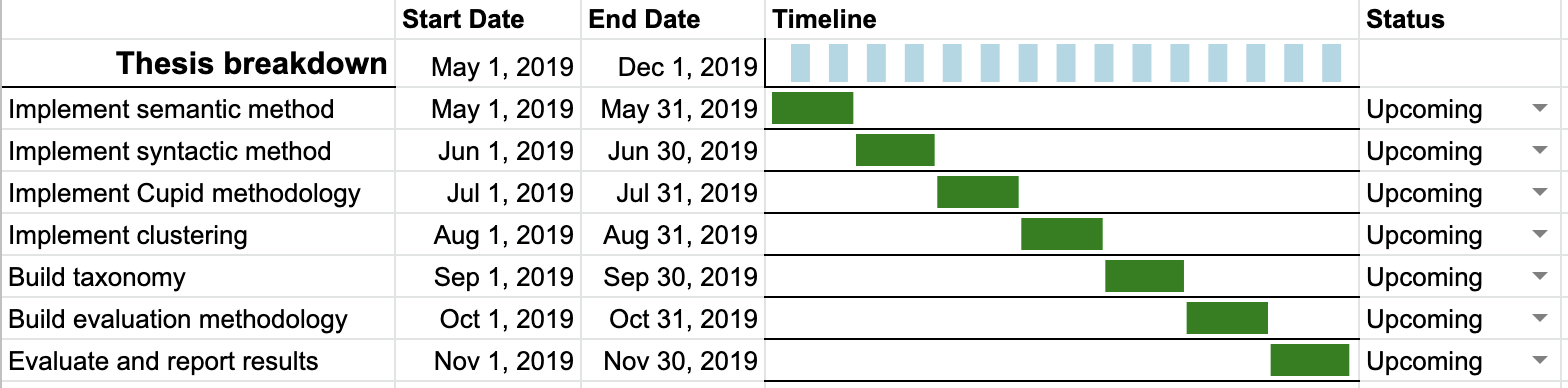
\includegraphics[width=0.9\textwidth] {figures/gantt.png}}}%
    \caption{Gantt chart with high-level tasks}
    \label{Figure:gantt}
\end{figure}


\printbibliography

%------------------------------------------------

\end{document}